\documentclass{article}
\usepackage{amsmath}
\usepackage{tikz}

\begin{document}
	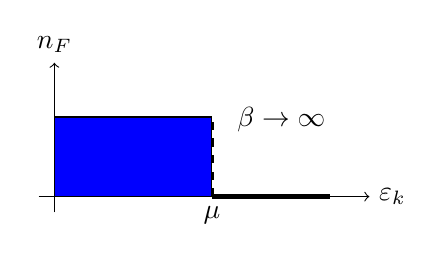
\begin{tikzpicture}
		\draw[->] (0,-0.2)--(0,1.7) node[above]{$n_F$};
		\draw[->] (-0.2,0)--(4,0) node[right]{$\varepsilon_k$};
		\draw[ultra thick] (0,1)--(2,1);
		\draw[ultra thick] (2,0)--(3.5,0);	
		\draw[ultra thick,dashed] (2,0)--(2,1);
		\node [below] at (2,0) {$\mu$};
		\draw [fill=blue] (0,0) rectangle (2,1);
		\node [above right] at (2.2,0.7) {$\beta\rightarrow\infty$};
	\end{tikzpicture}
\end{document}